\documentclass[a4paper,twocolumn,fleqn]{article}
\usepackage{ist,textcomp, amsmath}

\title{Reconstruction of 3D Objects with Radial Imaging}
\author{Daniel Filipe Nunes Silva, EPFL}

\begin{document}
\maketitle
\thispagestyle{empty}

\begin{abstract}
Objects have to be captured from various viewpoints to be reconstructed in 3D. This is traditionally done by moving the camera or by using multiple cameras. The purpose of this project is to get a similar result using a static system composed of one single camera and a hollow cylinder mirrored on the inside. Images are taken by the camera looking through the cylindrical mirror. As a result, the scene, which is located on the other side of the cylinder with respect to the camera, is captured directly and after reflection on the mirror sides. Hence we get multiple viewpoints within the same image.
\end{abstract}

\section{System}
The system is composed of a traditional camera and a hollow cylinder. Figure 1 shows the setup used for this project. The interior of the cylinder has to be reflective, ideally it should be a perfect mirror. Dimensions are discussed in the section properties. The cylinder must be rigidly fixed in front of the camera so that nothing can move once adjusted. This can be used to capture a scene from multiple viewpoints because the field of view of the camera is splitted into two parts. The inner part represents the scene directly captured while the outer part represents the scene after being reflected by the cylinder. The purpose of this paper is to reconstruct texture in 3D using this simple hardware. It is less expensive than using multiple cameras and there is no need to synchronize them.It does not require the knowledge of the camera's motion and could be used to capture moving scenes, as it is rigid and used as a single object. This kind of system can be extended by replacing the mirror. For example, a cone can be used instead of the cylinder to increase the field of view and capture bigger objects.

\begin{figure}[!hb]
  \centering
  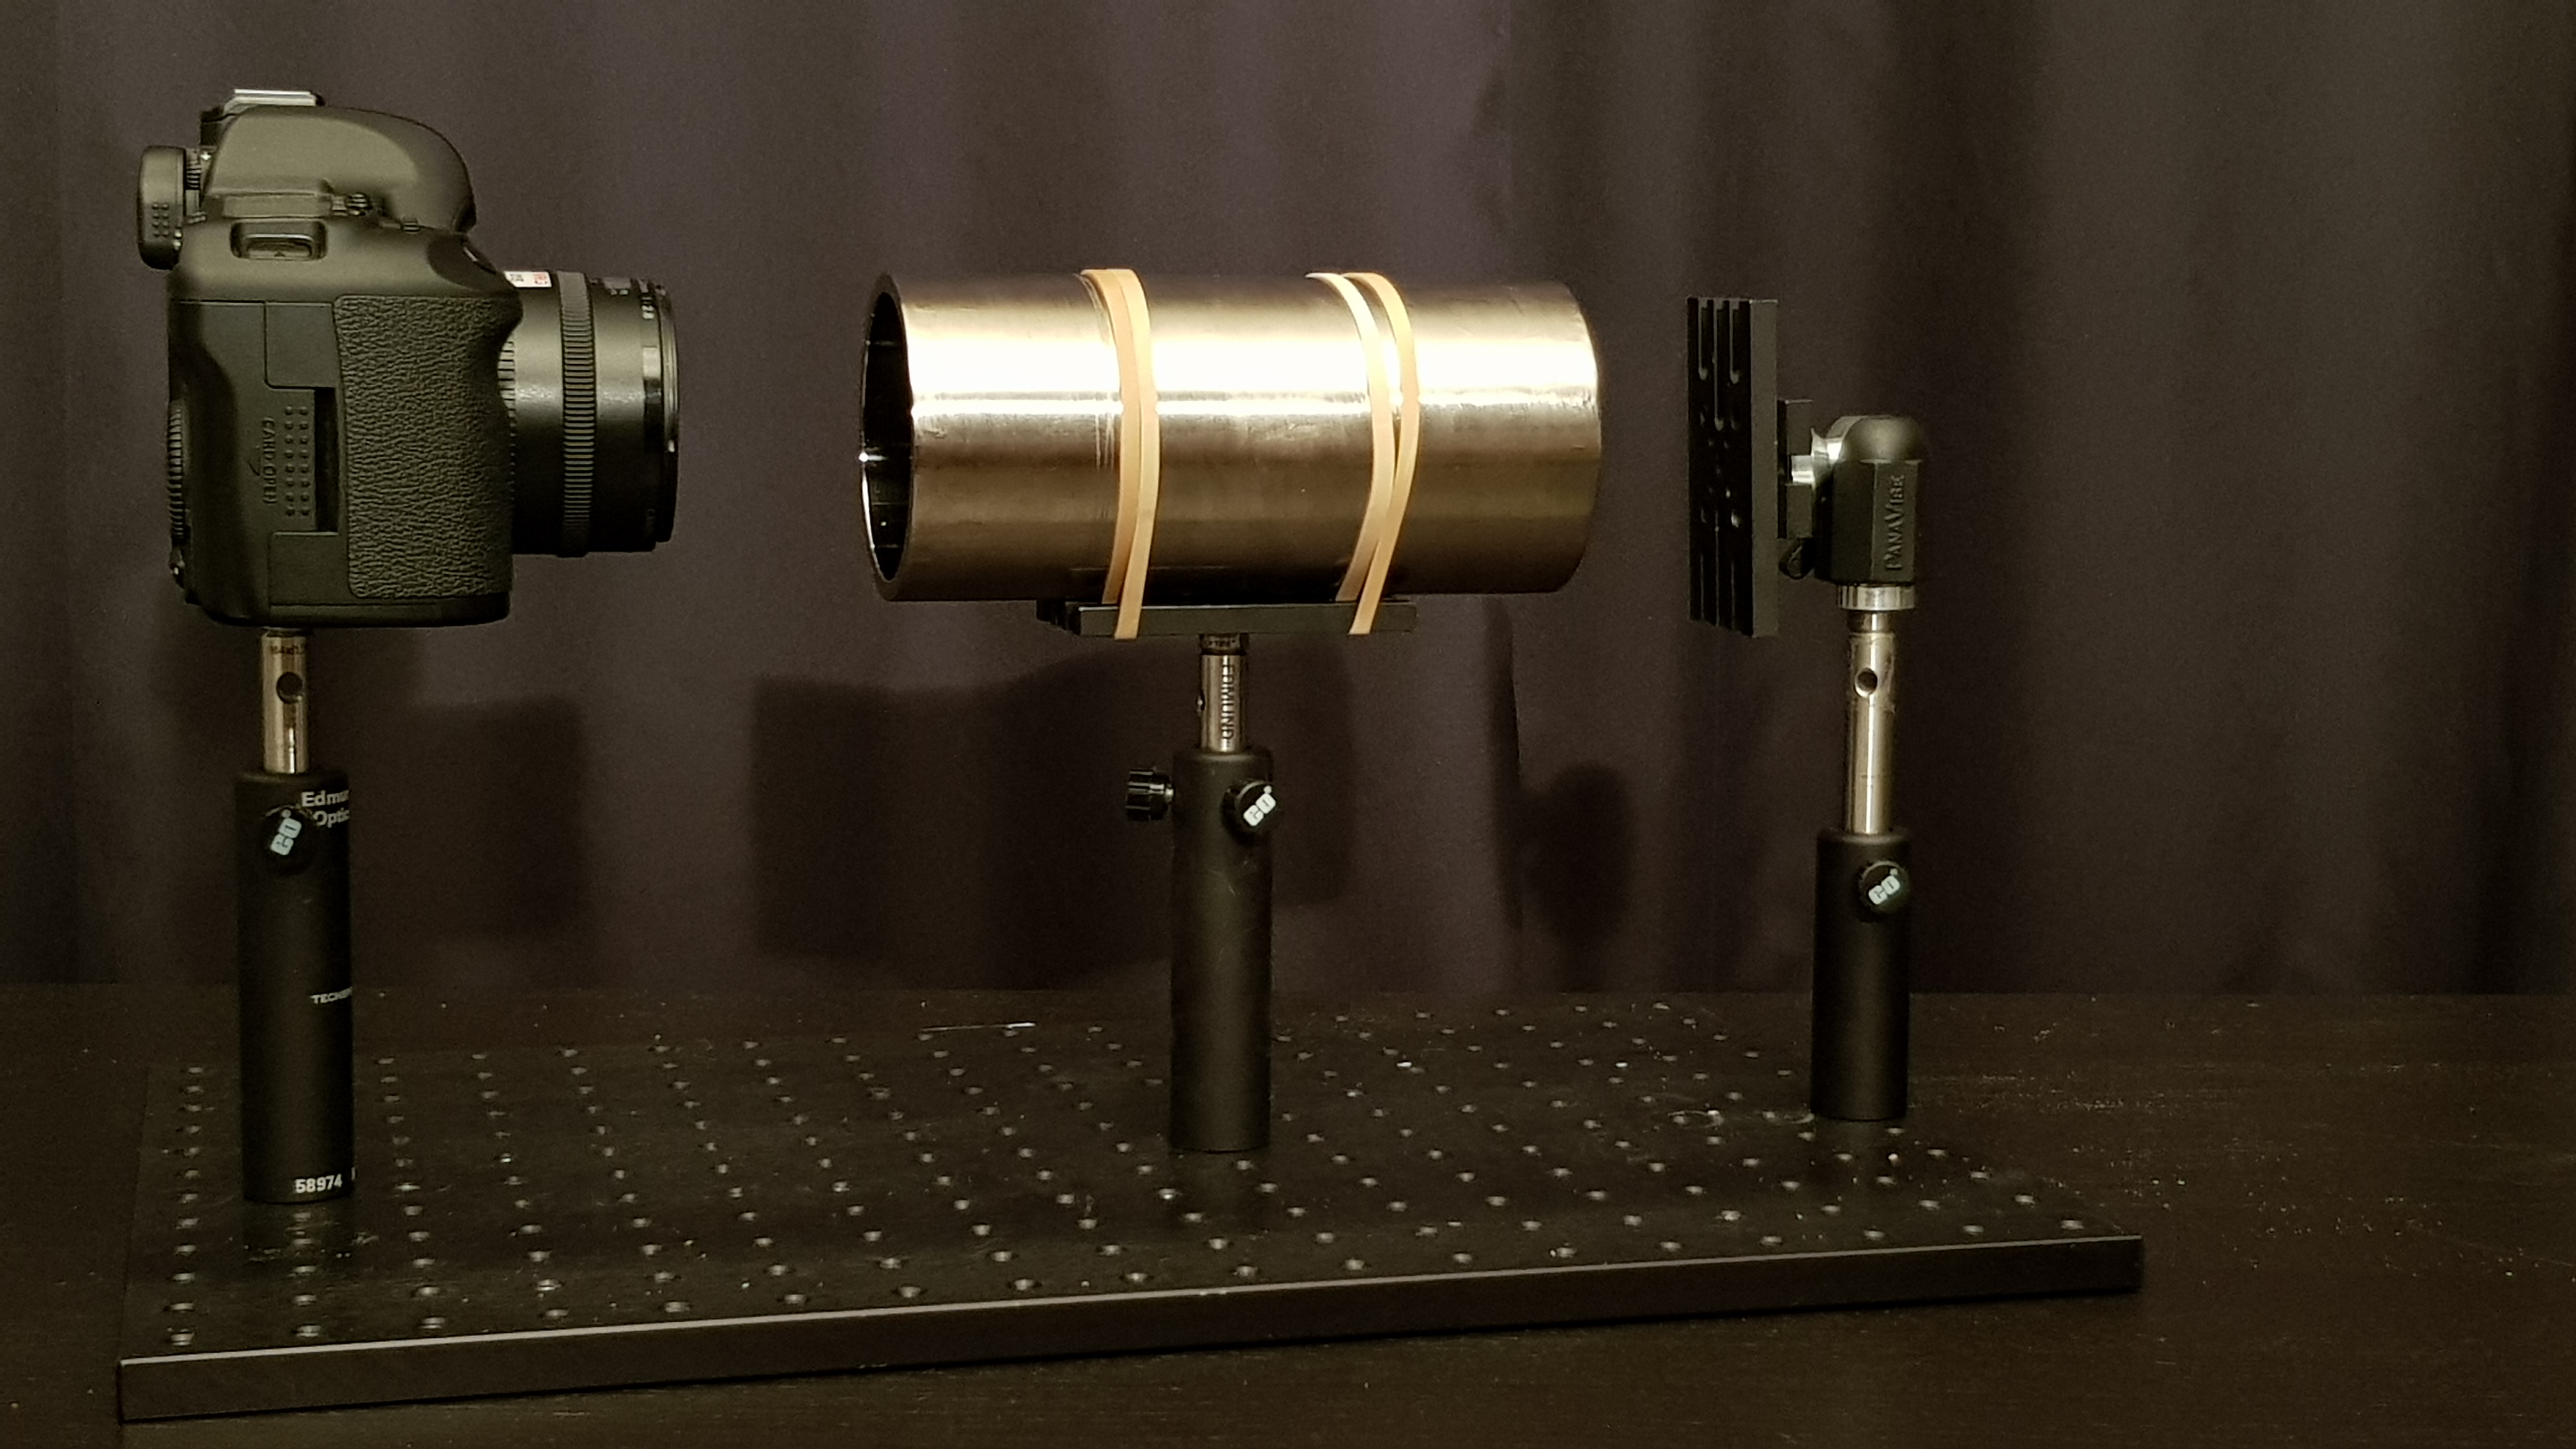
\includegraphics[width=1\columnwidth]{img/setup.jpg}
  \caption{Used Setup. The camera is a Canon 5D Mark II with a Canon EF 24mm f/2.8 lens. The cylinder has radius 35mm.}
\end{figure}

\section{Concept}
In order to take valid images with this system, the camera and the cylinder must be perfectly aligned : the optical axis of the camera should cross the cylinder in its center. The cylinder should have a specific length depending on its radius and on the camera field of view so that the scene is reflected only once. Figure 2 and 3 show two different slices of bread pictured with our setup. The directly captured part can be distinguished (inner circle) from the reflected one (outer annulus).

\begin{figure}[!b]
  \includegraphics[width=1\columnwidth]{img/bread01_sbs.png}
  \caption{Slice of bread 1, same image side by side}
  \includegraphics[width=1\columnwidth]{img/bread02_sbs.png}
  \caption{Slice of bread 2, same image side by side}
\end{figure}

Let's simplify the situation to understand the principle behind this by taking one horizontal slice of this image passing through the optical axis (Figure 5). We end up with a 1D vector, that can be cut into three parts : $AB$ - the left view; $BC$ - the central view; $CD$ - the right view. The segments $AB$ and $CD$ represent the virtual views and $BC$ is the real view. These virtual views are produced by the cylinder sides, that reflects the light coming from the scene into the camera sensor. This can also be seen as a main 1D camera capturing directly the $BC$ segment and two virtual cameras located on each side of the main one capturing the AC and $CD$ segments looking through the mirror sides. Hence, we get three different views of the same scene using only one camera.

The camera's locations are symmetric with respect to the optical axis. This operation is not limited to the horizontal line of the image but it can be reproduced by taking any radial slice passing through the center : the system is rotationally symmetric. This means that epipolar lines are radial. The idea is to extract a continuum of these radial lines and make them horizontal. Then, traditional algorithms can be used to recover the tridimensional values of the points. Thus, this kind of system can be called radial imaging system.

\begin{figure*}[!ht]
  \includegraphics[width=2\columnwidth]{img/complete2.png}
  \caption{Diagram of the system. Trinocular part in blue.}
\end{figure*}

\begin{figure}[!hb]
  \centering
  \includegraphics[width=0.8\columnwidth]{img/circle2.png}
  \caption{The inner circle corresponds to the real view, while the virtual views compose the outer annulus.}
\end{figure}

\section{Properties}
The first part describes how to compute values and dimensions related to the hardware. Then, we analyse intrinsic values of the system.

\subsection{Hardware}
This imaging system is entirely described by two parameters : the camera field of view $\alpha$ and the cylinder radius $r$. The distance $d$ between the focal point and the nearest end of the cylinder should be chosen in order to maximize the use of the camera field of view [1].

\begin{equation}
d = r \cdot \frac{\cos{(\alpha/2)}}{\sin{(\alpha/2)}}
\end{equation}

The length of the cylinder should ideally be $l$ to maximize the trinocular space. The trinocular space is the part of the scene visible from the three viewpoints. A longer length would produce multiple reflections : a point could be reflected sequentially on both sides of the mirror before hitting the camera sensor. This could be useful for other applications but it would restrict the trinocular space in our case. A shorter length would also restrict the trinocular space because the virtual views would converge closer [1].

\begin{equation}
l = 2 \cdot r \cdot \frac{\cos{(\alpha/2)}}{\sin{(\alpha/2)}}
\end{equation}

\subsection{Intrinsic}
The first interesting property when using these ideal values for hardware is that ratio of a virtual view segment ($AB$ and $CD$) and the real view segment ($BC$) is equal to $1$. Therefore, cutting the radial slices becomes a straightforward operation : it has to be splitted into three equal parts.

The virtual viewpoints are an axial symmetry of the real viewpoint around the mirrors sides located at a distance of $r$. The baseline $b$ is the distance between the real viewpoint$V_r$ and the virtual viewpoints $V_{vl}$ and $V_{vr}$ [1].

\begin{equation}
  b = 2 \cdot r
\end{equation}

The field of view $\phi$ of a virtual view can be computed with the following formula [1].

\begin{equation}
\phi = \arctan (\frac{\sin{(\alpha)}}{\cos(\alpha) + 2})
\end{equation}

The field of view $\psi$ of the real view can be computed with the following formula [1].

\begin{equation}
\psi = \alpha -2 \cdot \phi
\end{equation}

As the two virtual views converge in front of the camera, it is useful to compute the closest and the furthest trinocular point.

\begin{equation}
p_{closest} = 2 \cdot d \newline
p_{furthest} = 2 \cdot (d + l)
\end{equation}

The trinocular space increases linearly between the $p_{closest}$ until reaching the cylinder edges. Then it decreases linearly until $p_{furthest}$. Any point located in this space will appear on the three views. The real view can be combined with the two virtual views to estimate the 3D position of each point. Having three views allows us to use them pairwise for the reconstruction.

\section{Reconstruction}
In this section, the algorithm pipeline is discussed.

\subsection{Used Setup}
The camera has a full-frame sensor (24 $\times$ 36mm) and is combined with a 24mm lens. It captures 3744 $\times$ 5616 pixels jpg images. The field of view of this device is about 53 $\times$ 73\textdegree. In this application, only the minimum of these two values is useful because we are interested in square images.

The cylinder has radius 35mm and length 170mm. It is made out of brass, and the inside is polished and nickel plated. It is reflective but not a perfect mirror : it has some imperfections. In practise, it is hard to get a such mirror since it has to be as reflective as possible.

Images are taken by aligning everything manually. The system can be first roughly adjusted. Once the scene is in focus, the camera and the cylinder can be slightly moved so that the captured image has the correct proportions of viewpoints.

Our cylinder was longer than the ideal maximum length so it had to be put closer to the camera. We only used the needed length : the exceeding part of it is out of the field of view.

\begin{table}[!ht]
\caption{Properties of the used setup}
\begin{center}
\begin{tabular}{|p{0.4\columnwidth}|p{0.40\columnwidth}|}
\hline
Field of View $\alpha$ & 53.13\textdegree $\simeq$ 0,9272 $rad$ \\ \hline
Radius $r$ & 35 mm \\ \hline
Distance $d$ & 70 mm \\ \hline
Length $l$ & 140 mm \\ \hline
Baseline $b$ & 70 mm \\ \hline
Virtual field of view $\phi$& 17.10\textdegree $\simeq$ 0.2984  $rad$ \\ \hline
Real field of view $\psi$& 18.92\textdegree $\simeq$ 0.3302 $rad$ \\ \hline
Trinocular point $p_{closest}$ & 140 mm \\ \hline
Trinocular point $p_{furthest}$ & 420 mm \\ \hline
\end{tabular}
\end{center}
\end{table}

\subsection{Images}
The first step is to remove distortion introduced by the camera and the lens. This can be done by calibrating the camera with a chequerboard. Then the image should be cropped into a square. The two concentric circle must have the correct proportions (Figure 5). The square images have resolution 3744 $\times$ 3744 pixels.

\subsection{Views Separations}
Radial lines should be extracted and splitted into three parts. Then, they are stacked horizontally. We get three stacks of epipolar lines. Each segment has length $3744 / 3 = 1248$ pixels. In practise, the continuum of radials slices is limited by the camera's sensor pixel density. For convenience, only 1872 slices were extracted : the produced images are better proportioned ($1872 \times 1248$ pixels). Otherwise, image are too tall and difficult to visualize but preciser.

First, $2\pi$ (the full circle) should be discretized : $\gamma = 2\pi \div 1872 \simeq 0.003356$ $rad$ per slice. $\gamma$ is the angle between two consecutive slices. We should iterate over the 1872 slices and store their three segments in separate images. $\gamma_{n} = n \times \gamma$ is the angle made by the n-th slice with the positive $x$-axis.

Then, we assume that the image is stored in an 2D array $I$ indexed from (0, 0) to (3743, 3743). Three 2D array of $1872 \times 1248$ should be allocated : $V_{left}$, $V_{center}$, $V_{right}$. The first slice $s$ is the horizontal line in the middle of the image indexed by (1871, 0 to 3743). The first segment of $s$ indexed from 0 to 1247 is stored in $V_{left}$ at index (0, 1247 to 0), the second one indexed from 1248 to 2495 is stored in $V_{center}$ at index (0, 0 to 1247) and the third one indexed from 2496 to 3743 stored in $V_{right}$ at index (0, 1247 to 0). The reason why virtual views index are written backwards is that they are flipped by the mirror after being reflected.

More generally the n-th slice is stored at the n-th line of arrays $V$.

The index of the next slices should be computed according to $\gamma_{n}$. First, $sin_{n} = \sin{(\gamma_{n})}$ and $cos_{n} = \cos{(\gamma_{n})}$ are required. The slice $s_{n}$ is built in two steps : from index 0 to 1870 and from index 1872 to 3743. The point in the middle of $I$ is common for all slices. It appears at index 1871. The vector $s_n$ can be filled as follows for $1 \leq i \leq 1871$ :

\begin{center}
$
\begin{cases}
  s_n[1871 - i] = I[1871 + sin_n \cdot i][1871 - cos_n \cdot i]\\
  s_n[1871 + i] = I[1871 - sin_n \cdot i][1871 + cos_n \cdot i]
\end{cases}
$
\end{center}

The value at these index must be interpolated because they are not integer. Then, $s_n$ can be cut into three equal parts, which are stored in $V_{left}$, $V_{center}$, $V_{right}$.

After doing this for all $0 \leq n \leq 1871$, we have three stacks of horizontal epipolar lines :  $V_{left}$, $V_{center}$, $V_{right}$. These images should not be interpreted as actual images since they make no sense. They are built for the single purpose of allowing us to use traditional algorithms for 3D reconstruction.

\begin{figure}[!hb]
  \centering
  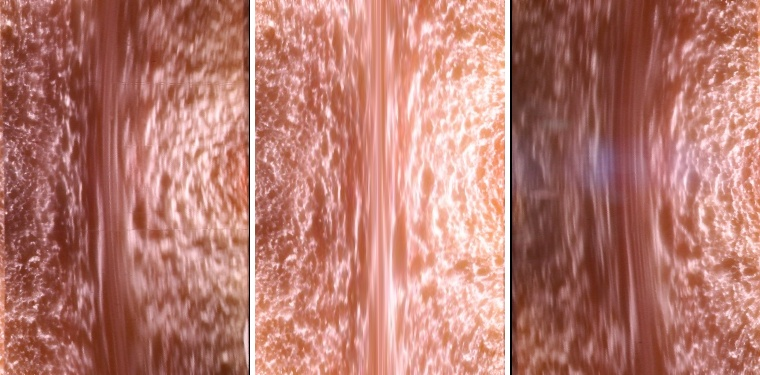
\includegraphics[width=1\columnwidth]{img/bread01_merged.JPG}
  \caption{Left, central and right views of bread 1}
\end{figure}

\begin{figure}[!hb]
  \centering
  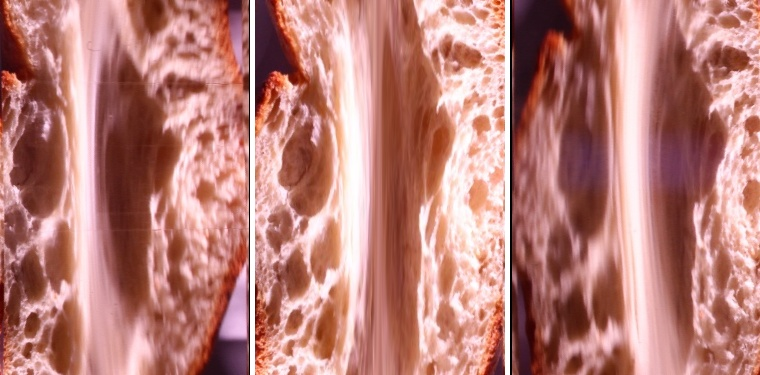
\includegraphics[width=1\columnwidth]{img/bread02_merged.JPG}
  \caption{Left, central and right views of bread 2}
\end{figure}

\subsection{Stereo matching}
Now, we can look for similarities along horizontal lines. $V_{center}$ is used as the reference. Normalized cross-correlation method is used for comparison on square windows of side $w=9$. For each line $l$ of $V_{center}$ and for each index $i$, we take the template $V_{center}[l:l+w][i:i+w]$ and we compare it with $V_{left}[l:l+w]$ and $V_{right}[l:l+w]$. The index $i'_{left}$ and $i'_{right}$ maximizing the comparison method between $V_{center}[l:l+w][i:i+w]$ and $V_{left}[l:l+w, i'_{left}:i'_{left}+w]$ and $V_{right}[l:l+w, i'_{right}:i'_{right}+w]$ are stored in 2D arrays : $C_{left}[l][i] $ and $C_{right}[l][i]$. Disparities can be computed for both $V_{left}$ and $V_{right}$ and stored as follows : $D[l][i] = i-i'$. Notice that each point in $V_{center}$ can be associated with another one in $V_{left}$ and $V_{right}$. This is only true for texture located at the end of the cylinder. The trinocular space shrinks as we go further than the end of the cylinder. Then, the three fields of view do not cover the same part of the scene. Hence, the object should be imaged as close as possible to the cylinder.

We can estimate the distance of the texture with respect to the cylinder prior to performing stereo matching. This reduces noise and avoids skewed values for disparities. The values of $D_{right}$ have to be positive. Otherwise, it would mean that our object is inside the cylinder. Moreover, if we know that the object is being captured from $0$ to $3$cm behind the cylinder, the disparity can be bounded according to Figure 8. This makes the computation more efficient as we look for plausible values in a restricted range. Values of $D_{right}$ are therefore bounded between $0$ and $164$ (Figure 9).

\begin{figure}[!t]
  \centering
  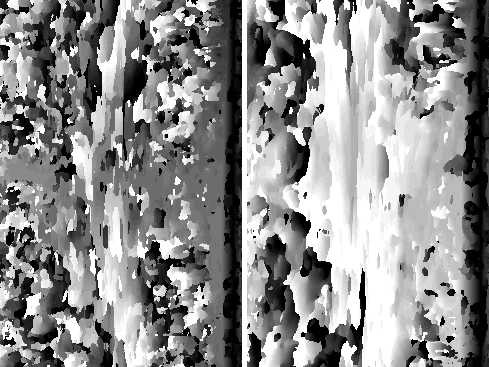
\includegraphics[width=0.8\columnwidth]{img/disp_map.png}
  \caption{$D_{right}$ for bread 1 (left) and bread 2 (right), disparities are bounded between 0 (white) and 164 (black).}
\end{figure}

\subsection{Triangulation}
Triangulation is about estimating the 3D coordinates of a point. This is done by throwing rays from the cameras' focal points through the corresponding pixels on the images and estimate their intersection.

The geometry of the system is described by the intrinsic and extrinsic parameters of each camera. The matrices $C_{left}$ and $C_{right}$ describe the pairs of pixels.

The triangulation procedure can be simplified by noticing that y-coordinates of $V_{left}$, $V_{center}$, $V_{right}$ are arbitrary. In fact, each horizontal line of these arrays represent a viewpoint of a 1D vector of points. These points lie on the 2D plane made by the optical axis and the radial line, where they are pictured. Therefore, triangulation can be done in 2D independently of $n$ (y-axis value).

The parameters are determined as if there were three similar cameras on the same plane looking along the z-axis.

The intrinsic parameters are the focal length in pixels $3744 \cdot 24 / 24 = 3744$ (sensor resolution [px] $\cdot$ focal length [mm] / sensor size[mm]) and the center of the image $3744 / 2 = 1872$.  This gives the following matrix. The same is used for the three views.

\begin{center}
$Cam_{Intrinsic} =
\begin{bmatrix}
3744 & 0 & 1872\\
0 & 3744 & 1872\\
0 & 0 & 1
\end{bmatrix}$
\end{center}

The extrinsic parameters describe the position of the camera in the real world. They are different for each camera since these do not point in the same direction from the same location. The real camera is at the origin, while the virtual ones are translated along the x-axis by $\pm 70$mm. The three cameras point in the same direction. We simply use different parts of their fields of view.

\begin{center}
$Cam_{Extrinsic-center} =
\begin{bmatrix}
1 & 0 & 0 & 0\\
0 & 1 & 0 & 0\\
0 & 0 & 1 & 0
\end{bmatrix}$

$Cam_{Extrinsic-left} =
\begin{bmatrix}
1 & 0 & 0 & 70\\
0 & 1 & 0 & 0\\
0 & 0 & 1 & 0
\end{bmatrix}$

$Cam_{Extrinsic-right} =
\begin{bmatrix}
1 & 0 & 0 & -70\\
0 & 1 & 0 & 0\\
0 & 0 & 1 & 0
\end{bmatrix}$
\end{center}

$C_{left}$, $C_{right}$ and the index of the the real view pixels must be adjusted to work with these matrices. The segments $BC$ stored in $V_{center}$ should be indexed from $1248$ to $2495$ since they are captured in the central third of the sensor : they lie in the central part of the field of view. The $AB$ segments stored in $V_{left}$ are captured left third of the sensor. This is equivalent as being captured by the right third of the left camera by axial symmetry around the mirror side. Hence, they should be shifted by 2495 pixels. Similarly, the right third corresponding to the $CD$ segments is equivalent to the left third of the right camera. The $i_{left}$, $i_{center}$, $i_{right}$ have the following structure in order to be triangulated correctly :

\begin{center}
$i_{left} :
\begin{smallmatrix}
[2496+disp_{2496} & 2497+disp_{2497} & ... & 3743+disp_{3743}]
\end{smallmatrix}$

$i_{center} :
\begin{smallmatrix}
[1248 & 1249 & ... & 2495]
\end{smallmatrix}$

$i_{right} :
\begin{smallmatrix}
[0+disp_0 & 1+disp_1 & ... & 1247+disp_{1247}]
\end{smallmatrix}$
\end{center}

These matrices are ready to be plugged in a triangulation function provided by most of the computer vision libraries. We end up with a 3D point cloud, whose points have the coordinates $(x, 0, z)$. Hence, the multiple slices cannot be distinguished.

\begin{figure}[t]
  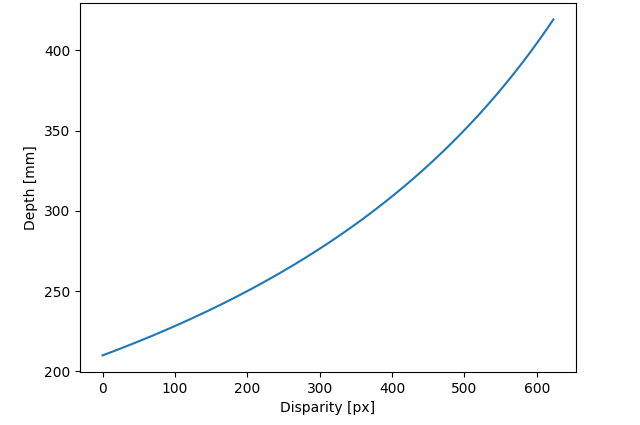
\includegraphics[width=1\columnwidth]{img/depth_disp.png}
  \caption{Depth a of a point computed by performing triangulation for every disparity.}
\end{figure}

\subsection{Shape Recovery}
The triangulated points coordinates should be rotated around the z-axis to recover the initial shape. This is done by changing the $x$ and $y$ coordinates of the points according to their index. Point from the n-th line should be updated as follows : $p_{n} = (c_{n} \cdot x, s_{n} \cdot x, z)$

\section{Results}
The results are not convincing. The left and right reconstructions are not consistent. This may be explained by the blur on the virtual views. The light is not uniformly reflected on the sides of the mirror. Diffraction makes the virtual views sharp on one side and blurry on the other : the light rays are spread variously depending on the angle of incidence. This affects every steps of the reconstruction. In particular, the stereo matching is less precise. This system seems to suffer from a inherent weakness despite its elegance.

\begin{figure}[!ht]
  \centering
  \includegraphics[width=1\columnwidth]{img/bread2_3d.png}
  \caption{Reconstruction of bread 2 with left and right views}
  \includegraphics[width=1\columnwidth]{img/bread1_3d.png}
  \caption{Reconstruction of bread 1 with left and right views}
\end{figure}

\section{Conclusion and Future Work}
In this project, we have built a system composed of a camera and an hollow cylinder mirrored on the inside. This allows us to capture multiple viewpoints within a single image. This image can therefore be used for 3D reconstruction. The algorithm to transform the taken images into a 3D point cloud has been implemented. A simple technique to make use of prior knowledge about the distance between the camera and the object has also been introduced in order to have a more plausible reconstruction.

In future work, other stereo matching method should be tested to deal with the blur on virtual views. With better reconstructions, it could be interesting to analyse the effective precision of this system comparing the left and the right reconstruction. Finally, we could design a similar system that would not be skewed by diffraction so that blur would be less important.

\small
\begin{thebibliography}{9}
\bibitem{bib1}Sujit Kuthirummal Shree K. Nayar, Multiview Radial Catadioptric Imaging for Scene Capture, Columbia University, 2006
\end{thebibliography}

\end{document}
